\documentclass{article}
\usepackage{graphicx} 
\usepackage{verbatim}

\title{Integration of Stata Outputs with {\LaTeX}}
\author{}
\date{}

\begin{document}

\maketitle

\section{Introduction}
This exercise demonstrates how to export files from Stata that can be read in {\LaTeX}, ensuring automatic updates whenever you execute Stata and {\LaTeX} codes.

\section{Setting up a Folder Structure}
Start by creating a folder named \texttt{Project}. Inside this folder, create two additional folders: \texttt{Output} and \texttt{Final}. The \texttt{Output} folder will serve as the destination for exporting tables and graphs from Stata. Later, you can import these files into your {\LaTeX} document. When starting a new {\LaTeX} project, ensure that the \texttt{.tex} file is saved in the \texttt{Final} folder before compiling. This step is necessary for {\LaTeX} to correctly interpret the file paths specified within the document. As your project expands, it is common to add sub-folders within the \texttt{Output} folder to organize your files. For instance, you may choose to create separate folders for tables and figures. You can tailor the organization to your preferences as you find the most suitable approach.

\section{Exporting Figures and Tables in Stata}
All figures produced in Stata can be exported in \texttt{.png} format. The following code example demonstrates the creation of a scatterplot between car prices and mileages using Stata's auto.dta dataset. The resulting figure is saved as scatter.png in the \texttt{Output} folder.

\begin{verbatim}
clear all
global main_folder "Enter Your Folder Path Here"
sysuse auto.dta, clear
graph twoway scatter price mpg, name(scatter)
graph export "$main_folder/scatter.png", replace
\end{verbatim}

To export regression tables, you can utilize the \texttt{esttab} command in Stata. Start by clearing any existing results from memory by typing \texttt{estimates clear}. Then, run the desired regressions whose results you wish to export. If Stata can successfully run the regression and display its results in the Stata window, \texttt{esttab} will be able to export them to \texttt{.tex} format. This sample code demonstrates how to run multiple regressions and export their results using the \texttt{esttab} command:

\begin{verbatim}
// Running regression 1
qui reg price mpg
est sto m1

// Running regression 2
qui reg price mpg length
est sto m2

// Running regression 3
qui reg price mpg length rep78
est sto m3

// Exporting results to reg.tex using esttab
esttab m1 m2 m3 using "$main_folder/reg.tex", replace
\end{verbatim}

\section{Importing Results in {\LaTeX}}
After exporting the figures and tables from Stata, you can add their paths to your {\LaTeX} file and dynamically update them whenever you make any changes to your original Stata code.\\

\textbf{A sample code for importing a figure in {\LaTeX}} 
\begin{verbatim}
\begin{figure}
    \centering
    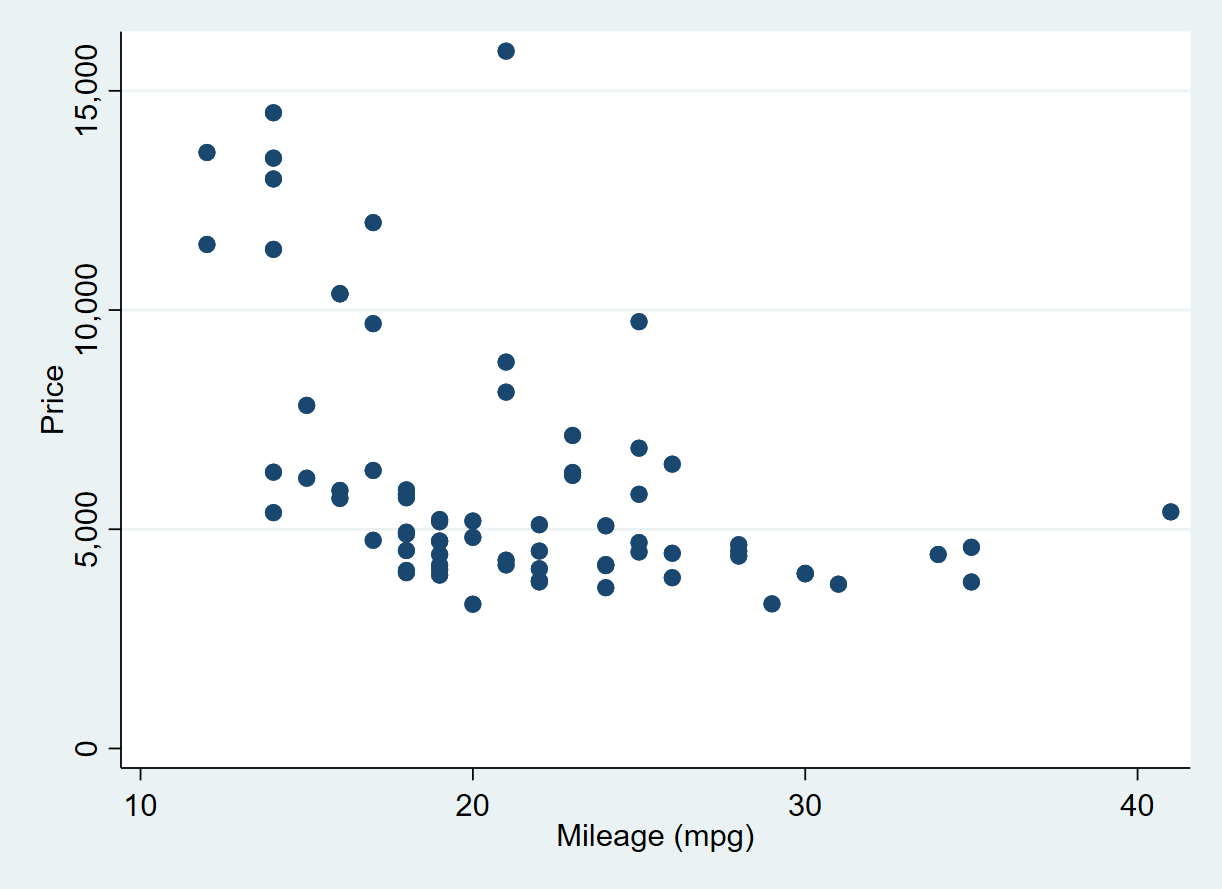
\includegraphics[width=0.7\linewidth]{D:/Project/Output/scatter.png}
    \caption{Scatterplot of Car Prices and Mileage}
\end{figure}
\end{verbatim}

\textbf{A sample code for importing a table in {\LaTeX}} 
\begin{figure}
    \centering
    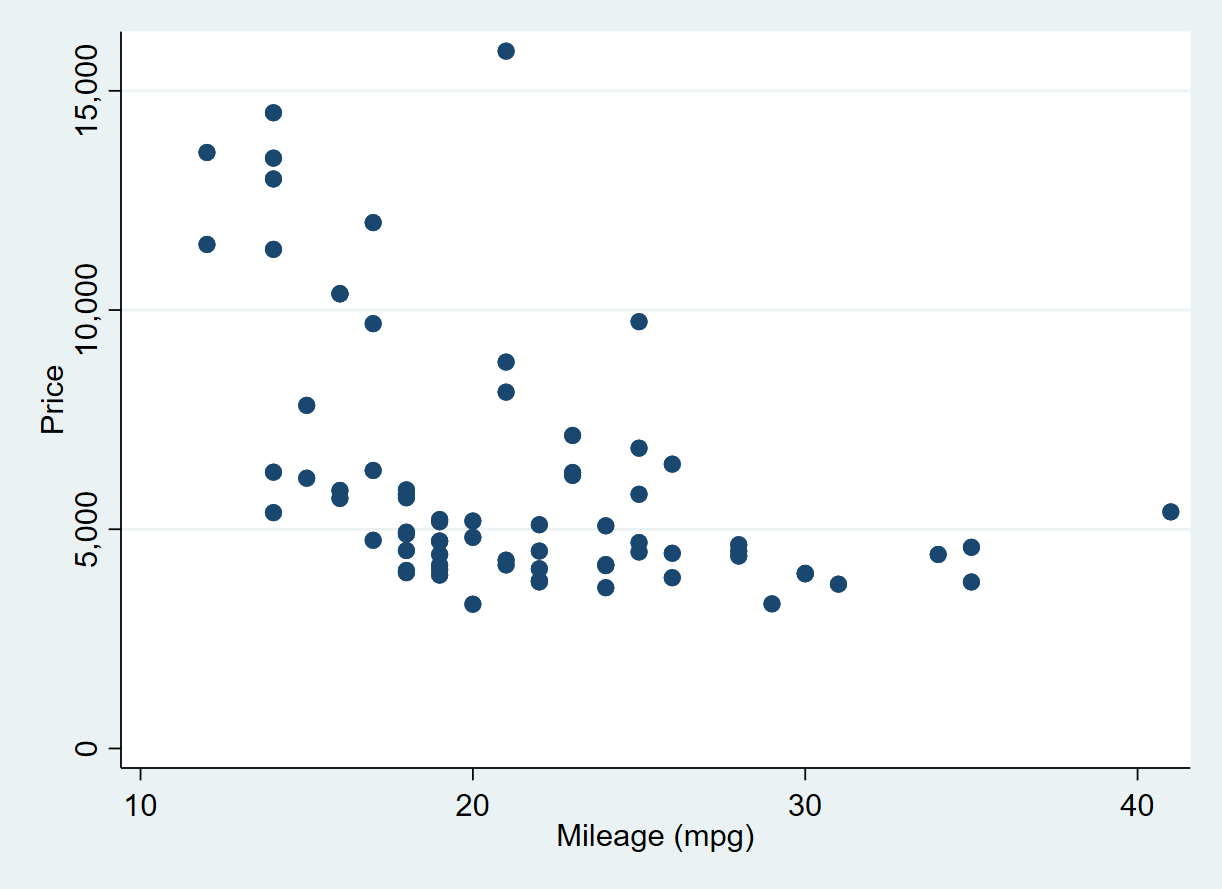
\includegraphics[width=0.7\linewidth]{D:/Project/Output/scatter.png}
    \caption{Scatterplot of Car Prices and Mileage}
\end{figure}

\begin{verbatim}
\begin{table}
    \centering
    \caption{Regression Results}
    {
\def\sym#1{\ifmmode^{#1}\else\(^{#1}\)\fi}
\begin{tabular}{l*{3}{c}}
\hline\hline
            &\multicolumn{1}{c}{(1)}&\multicolumn{1}{c}{(2)}&\multicolumn{1}{c}{(3)}\\
            &\multicolumn{1}{c}{price}&\multicolumn{1}{c}{price}&\multicolumn{1}{c}{price}\\
\hline
mpg         &      -238.9\sym{***}&      -173.7         &      -178.2         \\
            &     (-4.50)         &     (-1.98)         &     (-1.97)         \\
[1em]
length      &                     &       21.29         &       30.68         \\
            &                     &      (0.93)         &      (1.34)         \\
[1em]
rep78       &                     &                     &       698.3\sym{*}  \\
            &                     &                     &      (2.05)         \\
[1em]
\_cons      &     11253.1\sym{***}&      5864.3         &      1783.9         \\
            &      (9.61)         &      (1.00)         &      (0.30)         \\
\hline
\(N\)       &          74         &          74         &          69         \\
\hline\hline
\multicolumn{4}{l}{\footnotesize \textit{t} statistics in parentheses}\\
\multicolumn{4}{l}{\footnotesize \sym{*} \(p<0.05\), \sym{**} \(p<0.01\), \sym{***} \(p<0.001\)}\\
\end{tabular}
}

\end{table}
\end{verbatim}

\begin{table}
    \centering
    \caption{Regression Results}
    {
\def\sym#1{\ifmmode^{#1}\else\(^{#1}\)\fi}
\begin{tabular}{l*{3}{c}}
\hline\hline
            &\multicolumn{1}{c}{(1)}&\multicolumn{1}{c}{(2)}&\multicolumn{1}{c}{(3)}\\
            &\multicolumn{1}{c}{price}&\multicolumn{1}{c}{price}&\multicolumn{1}{c}{price}\\
\hline
mpg         &      -238.9\sym{***}&      -173.7         &      -178.2         \\
            &     (-4.50)         &     (-1.98)         &     (-1.97)         \\
[1em]
length      &                     &       21.29         &       30.68         \\
            &                     &      (0.93)         &      (1.34)         \\
[1em]
rep78       &                     &                     &       698.3\sym{*}  \\
            &                     &                     &      (2.05)         \\
[1em]
\_cons      &     11253.1\sym{***}&      5864.3         &      1783.9         \\
            &      (9.61)         &      (1.00)         &      (0.30)         \\
\hline
\(N\)       &          74         &          74         &          69         \\
\hline\hline
\multicolumn{4}{l}{\footnotesize \textit{t} statistics in parentheses}\\
\multicolumn{4}{l}{\footnotesize \sym{*} \(p<0.05\), \sym{**} \(p<0.01\), \sym{***} \(p<0.001\)}\\
\end{tabular}
}

\end{table}

\newpage
\section{Editing a \texttt{.tex} File in Stata After Exporting}
Sometimes, after exporting figures and tables from Stata to \LaTeX, you may need to make changes or edits to the generated \texttt{.tex} files. Stata provides a useful command called \texttt{filefilter} that allows you to modify the exported \texttt{.tex} files programmatically.

To edit a \texttt{.tex} file in Stata using the \texttt{filefilter} command, follow these steps:

\begin{enumerate}
  \item Open the \texttt{.tex} file you want to edit in a text editor and identify the patterns or text that you want to modify.
  \item In Stata, use the \texttt{filefilter} command to perform the necessary modifications. The basic syntax of the \texttt{filefilter} command is as follows:
  
  \texttt{filefilter [options] infile using outfile}
  
  \begin{itemize}
      \item \texttt{infile} is the path to the original \texttt{.tex} file.
      \item \texttt{using} specifies the modified \texttt{.tex} file's output path.
      \item \texttt{outfile} is the modified \texttt{.tex} file generated by \texttt{filefilter}.
  \end{itemize}
  
  \item Define the modifications using the appropriate options and execute the \texttt{filefilter} command. Stata will apply the specified modifications and generate the modified \texttt{.tex} file.
\end{enumerate}

Here is an example that demonstrates how to use the \texttt{filefilter} command to perform text replacements. The first line replaces all occurrences of \texttt{price} with \texttt{Price} and saves the new file as \texttt{reg\_temp.tex}. The second line replaces \texttt{mpg} with \texttt{Mileage} and saves the new file as \texttt{reg\_modified.tex}. Similarly, the third and fourth lines of the code perform replacements for \texttt{length} and \texttt{rep78}, respectively.

\begin{verbatim}
filefilter "$main_folder/reg.tex" "$main_folder/reg_temp.tex",
    from("price") to("Price") replace
filefilter "$main_folder/reg_temp.tex" "$main_folder/reg_modified.tex",
    from("mpg") to("Mileage") replace
filefilter "$main_folder/reg_modified.tex" "$main_folder/reg_temp.tex",
    from("length") to("Length") replace
filefilter "$main_folder/reg_temp.tex" "$main_folder/reg_modified.tex",
    from("rep78") to("Repair record") replace
\end{verbatim}

\begin{table}
    \centering
    \caption{Regression Results: Modified Table}
    {
\def\sym#1{\ifmmode^{#1}\else\(^{#1}\)\fi}
\begin{tabular}{l*{3}{c}}
\hline\hline
            &\multicolumn{1}{c}{(1)}&\multicolumn{1}{c}{(2)}&\multicolumn{1}{c}{(3)}\\
            &\multicolumn{1}{c}{Price}&\multicolumn{1}{c}{Price}&\multicolumn{1}{c}{Price}\\
\hline
Mileage         &      -238.9\sym{***}&      -173.7         &      -178.2         \\
            &     (-4.50)         &     (-1.98)         &     (-1.97)         \\
[1em]
Length      &                     &       21.29         &       30.68         \\
            &                     &      (0.93)         &      (1.34)         \\
[1em]
Repair record       &                     &                     &       698.3\sym{*}  \\
            &                     &                     &      (2.05)         \\
[1em]
\_cons      &     11253.1\sym{***}&      5864.3         &      1783.9         \\
            &      (9.61)         &      (1.00)         &      (0.30)         \\
\hline
\(N\)       &          74         &          74         &          69         \\
\hline\hline
\multicolumn{4}{l}{\footnotesize \textit{t} statistics in parentheses}\\
\multicolumn{4}{l}{\footnotesize \sym{*} \(p<0.05\), \sym{**} \(p<0.01\), \sym{***} \(p<0.001\)}\\
\end{tabular}
}

\end{table}

\end{document}
